\chapter[Instruções de utilização]{Instruções de utilização}
\label{cap:instrucoes}

O projeto está preparado para receber o caminho dos arquivos de código-fonte via linha de comando (terminal do Linux ou \textit{prompt} de comandos do Windows). A passagem dos argumentos pode ser configurada no ambiente de desenvolvimento de preferência ou informado na inicialização do arquivo executável .jar ou na execução direta dos arquivos .class. Exemplo de execução:

\begin{itemize}
    \item \textbf{Execução do .jar:} o seguinte comando deve ser executado na mesma pasta do arquivo .jar caso as configurações do projeto anexado sejam mantidas:
    
    \begin{center}
        \textbf{java -jar KPiler.jar test/test1.k test/test1.k}
    \end{center}

    \item \textbf{Execução dos arquivos .class:} deve-se navegar para a pasta do \textit{build} e executar os seguintes comandos para compilar e executar o código:
    
    \begin{center}
        \textbf{javac Parser.java}
        
        \textbf{java Parser test/test1.k test/test1.k}
    \end{center}

\end{itemize}


\begin{figure}[!h]
\label{fig:execution}
\centering
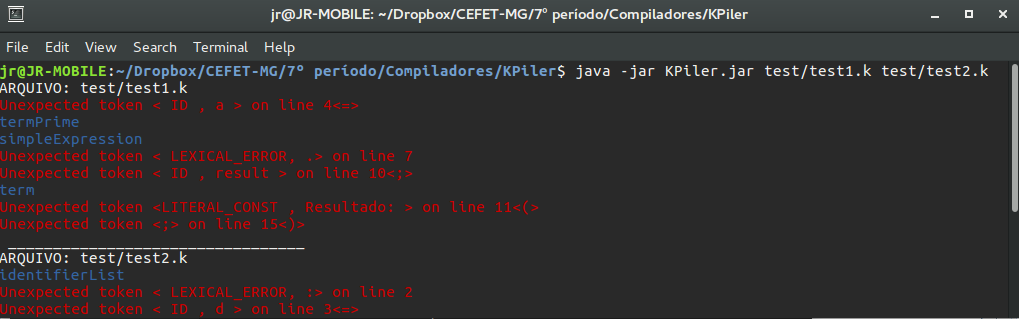
\includegraphics[width=16cm,height=20cm,keepaspectratio]{img/execution.png}
\caption{Execução do programa via terminal.}
\end{figure}